\documentclass[11pt]{article}
\linespread{1.25}

\usepackage[top = 2cm, right=2cm, left=2cm]{geometry}
\usepackage{graphicx}

\usepackage[section]{placeins}
\usepackage[hidelinks, urlcolor=blue]{hyperref}
\usepackage{float} % for image position in exatly where you want
\usepackage[perpage, stable]{footmisc}
\usepackage{amsmath}
\usepackage{titling}

\usepackage{xepersian}
\settextfont{B Nazanin}
\setlatinmonofont{CMU Serif}
%\setlatinmonofont{Times New Roman}
\setlatintextfont{Times New Roman}

% Set Latin Modern font for the bullets in itemizea
\newfontfamily\latinbullet{Latin Modern Roman}





% Commands
\newcommand{\column}[1]{\lr{\textit{#1}}}
\renewcommand{\labelitemi}{{\latinbullet\textbullet}} % Use the bullet from Latin Modern font

% Custom title page setup
\makeatletter
\def\maketitle{
	\begin{titlepage}
		\begin{center}
			\vspace*{2cm}
			
			{\Large\bfseries درس یادگیری ماشین\par}
			\vspace{2cm}
			
			{\Huge\bfseries گزارش تکلیف
				\lr{Backpropagation}\par}
			\vspace{3cm}
			
			{\large\bfseries استاد درس:\par}
			{\large دکتر افتخاری\par}
			\vspace{1.5cm}
			
			{\large\bfseries نگارش:\par}
			{\large امیرحسین ابوالحسنی\par}
			{\large شماره دانشجویی: 400405003\par}
			\vspace{2cm}
			
			\vfill  % pushes the date to bottom
			
			{\large\bfseries پاییز \lr{1403}}
			
		\end{center}
	\end{titlepage}
	\setcounter{page}{1}
}
\makeatother


\begin{document}
	\maketitle	
	\tableofcontents
	\newpage
	\section{مقدمه}
	الگوریتم پس انتشار خطا
	\footnote{\lr{Back Propagation}}،
	الگوریتمی برای یادگیری با نظارت در شبکه‌های عصبی با استفاده از گرادیان کاهشی است. در این روش، برای یک شبکه عصبی مصنوعی و تابع خطای مشخص،‌گرادیان تابع خطا نسبت به وزن‌های شبکه عصبی محاسبه می‌‌شود.\\
	در این تکلیف به پیاده سازی بلوک‌های سازنده یک شبکه عصبی پراخته می‌شود، و در هر بلوک، متد‌های مورد نیاز برای انجام الگوریتم پس انتشار خطا پیاده سازی می شود.
	\section{پیاده سازی لایه خطی}
	هر لایه از شبکه عصبی متشکل از تعدادی نورون می باشد که تعداد بعد ورودی را به تعداد بعد خروجی نگاشت می کند. پارامتر‌های مهمی که باید برای هر لایه ذخیره شود وزن‌های لایه‌ و بایاس لایه می‌باشد. همچنین گرادیان‌ها نسبت به وزن و بایاس نیز باید نگه داشته شود.\\
	برای هر لابه خطی سه متد در نظر گفته شده است:
	\begin{itemize}
		\item \lr{forward} :‌متدی که وظیفه انجام عمل پیشخور لایه را بر عهده دارد.
		\item \lr{backward} : متدی که وظیفه محاسبه گرادیان نسبت به وزن های این لایه را دارد.
		\item \lr{step}: متدی که وظیفه بروزرسانی وزن‌ها با توجه به گرادیان محاسبه شده را دارد.
	\end{itemize}
	\section{پیاده سازی توابع فعال‌سازی}
	برای پیاده سازی توابع فعال ساز، به آنها به شکل یک لایه نگاه کرده می‌شود. کلاس هر کدام از توابع فعال ساز متدهای زیر را پیاده‌سازی می‌کند.
	\begin{itemize}
		\item \lr{forward}: وظیفه این تابع محاسبه انجام عملیات تابع روی ورودی‌ها می‌باشد.
		\item \lr{backward}: محاسبه گرادیان خطا نسبت به ورودی
	\end{itemize}
	\subsection{تابع سیگموید}
	تابع سیگمویید
	\footnote{\lr{Sigmoid}}
	 به فرمول :
	\[ f(x) = \frac{1}{1 + e^{-x}} \]
	ورودی را به بازه $[1, 0]$ نگاشت می‌کند و برای انجام دسته‌بندی دو کلاسه مورد استفاده قرار می‌گیرد.\\
	یکی دیگر از دلایل استفاده از سیگمویید، سادگی در محاسبه مشتق آن است.
	\[ f'(x) = f(x)\cdot (1 - f(x)) \]
	\newpage
	\subsection{تابع واحد یک‌سو شده خطی}
	تابع 
	\lr{ReLU}
	با فرمول 
	\[ f(x) = \max (0, x )\]
	سعی در ایجاد روابط غیر خطی در شبکه دارد.
	همچنین مشتق این تابع به سادگی محاسبه می‌گردد:
	$$ f'(x) = \begin{cases} 1 & x > 0 \\ 0 & \text{\lr{otherwise}} \end{cases} $$
	\subsection{
		تابع
		\lr{Softmax}
	}
	تابع 
	\lr{Softmax}
	به فرمول:
	\[ f(x_i) = \frac{e^{x_i}}{\sum_{j = 1}^{n} e^{x_j}} \]
	به طور عمده برای دسته‌بندی با بیش از دو کلاس مورد استفاده قرار می‌گیرد.
	\section{پیاده سازی توابع هزینه}
	برای پیاده‌سازی هر تابع هزینه مقادیر $y$ و $\hat{y}$ در کلاس، نگهداری می‌شود.
	همچنین متد‌های زیر در هر کلاس پیاده‌سازی می‌شود:
	\begin{itemize}
		\item \lr{forward} : این متد ارور را با توجه به رابطه تعریف شده برای تابع هزینه محاسبه می‌کند.
		\item \lr{backward} : این متد مشتق تابع هزینه نسبت به $\hat{y}$
		را محاسبه می‌کند.
	\end{itemize}
	\section{پیاده‌سازی شبکه}
	یک کلاس برای یک شبکه پرسپترون چند لایه
	\footnote{\lr{MLP}}
	 نوشته می شود که در آن حلقه آموزش و متد‌های مورد نیاز برای پیشخور و پس انتشار خطا پیاده سازی می‌گردد.
	\section{آموزش شبکه}
	شبکه
	\lr{MLP}
	پیاده سازی شده،
	بر روی دیتاست 
	\lr{Fashion MNIST}
	و کلاس‌های 
	\lr{T-shirt/top}
	و
	\lr{Trouser}
	و
	\lr{Sneaker}
	آموزش دیده است.
	کانفیگ آموزش در جدول
	\ref{tbl: train config}
	نشان داده شده است.
	\begin{table}[H]
		\centering
		\begin{tabular}{|c|c|}
			\hline
			نوع & مقدار\\
			\hline
			تعداد لایه‌ها & 3\\
			\hline
			\lr{Epoch} & 30\\
			\hline
			نرخ یادگیری & $10^{-3}$\\
			\hline
			سایز \lr{Batch} & 64\\
			\hline
			تابع هزینه & \lr{Cross Entropy}\\
			\hline
		\end{tabular}
		\caption{کانفیگ آموزش شبکه}
		\label{tbl: train config}
	\end{table}
	\begin{figure}[H]
		\centering
		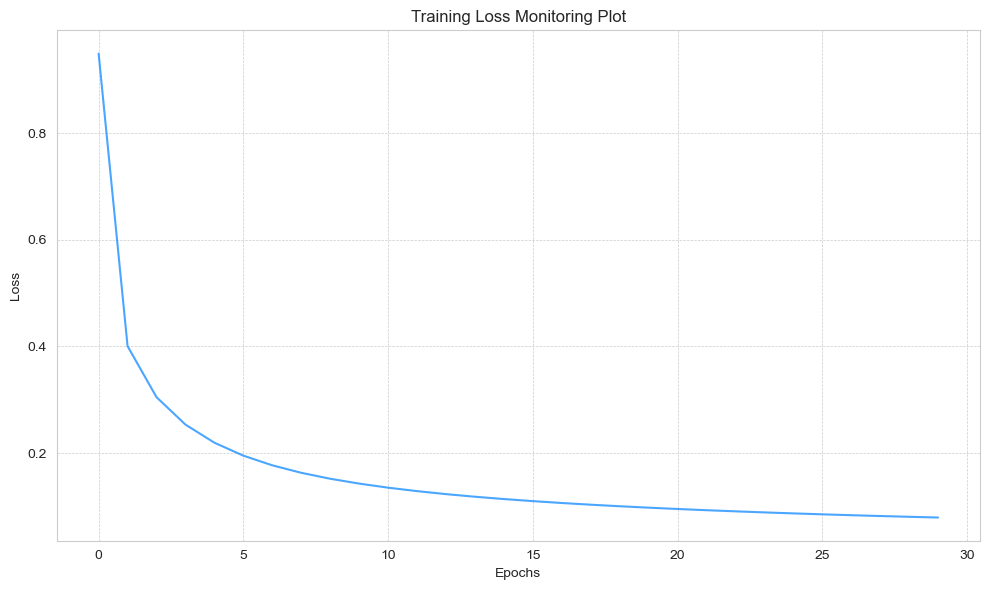
\includegraphics[scale=0.6]{figs/train_mlp_loss}
		\caption{نمودار روند خطای آموزش در طول یادگیری}
		\label{fig: train loss}
	\end{figure}
	\section{ارزیابی و نتایج}
	مدل پس از آموزش به دقت
	98\%
	رسید. همچنین نمونه‌ای از خروجی مدل در شکل
	\ref{fig: output}
	مشاهده می شود.\\
	\begin{figure}[H]
		\centering
		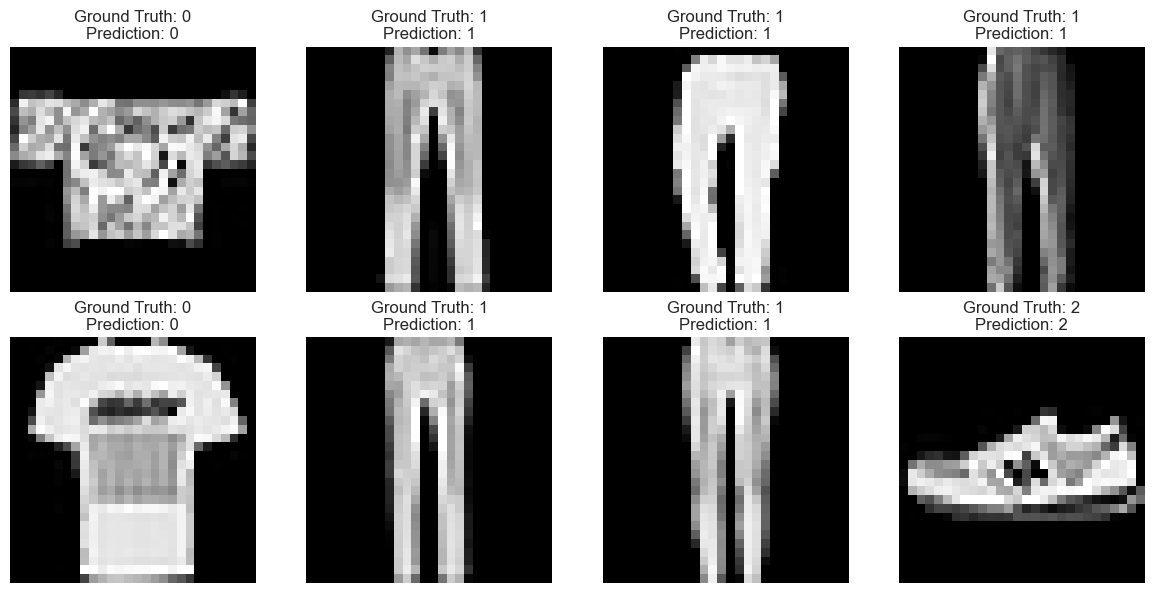
\includegraphics[scale=0.5]{figs/output}
		\caption{نمونه ای از دیتاست و خروجی مدل}
		\label{fig: output}
	\end{figure}
	با بررسی ماتریس سردرگمی
	\footnote{\lr{Confusion Matrix}}
	(
	شکل
	\ref{fig: conf mat}
	)
	متوجه می‌شویم که مدل به خوبی توانسته هر سه کلاس را یادگیری کرده و داده‌های تست را به خوبی دسته بندی کند. از این موضوع می‌توان نتیجه گرفت که پیاده سازی هایی که انجام شده صحیح بوده و مشکلی در آنها وجود نداشته است.
	\begin{figure}[H]
		\centering
		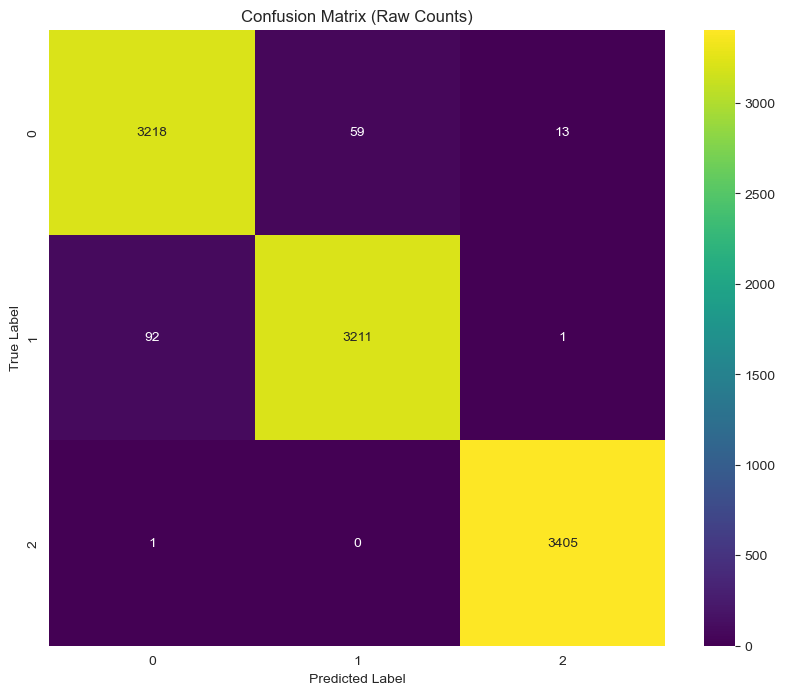
\includegraphics[scale=0.6]{figs/confMat}
		\caption{ماتریس سردرگمی}
		\label{fig: conf mat}
	\end{figure}
	
	
	
	
	
	
	
	
	
	
	
	
	
	
	
	
	
	
	
	
	
\end{document}